Für die Versendung des Dokuments werden nach der Vereinigung der Komponenten der Dokumentendatei zusätzlich der öffentliche Signaturschlüssel und das Zertifikat des Signaturschlüssel-Inhabers angehängt und versendet. Anhand des Zertifikates kann die Identitätsprüfung des Absenders durchgeführt werden. Die Bestandteile des Zertifikates sind der Name bzw. das Pseudonym des Signaturschlüssel-Inhabers, die Zertifizierungsstelle und deren Identifizierungsnummer, das Ausstellungsdatum sowie die Gültigkeitsdauer und der öffentliche Signaturschlüssel mit dem verwendeten Hash-Algorithmus. \cite{techno1}\cite{techno4}
\begin{figure}[!ht]
    \centering
    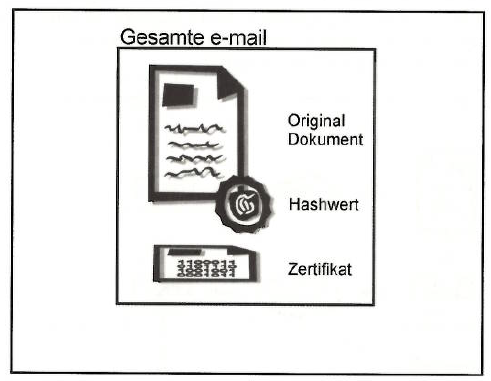
\includegraphics[height=220pt, width=300pt]{versand_doc.PNG}
    \caption[Aufbau versandfertiges Dokument]{\small{Aufbau versandfertiges Dokument \cite{techno6}}}
\end{figure}